\documentclass{standalone}
\usepackage{tikz}
\usetikzlibrary{shapes}
\begin{document}

    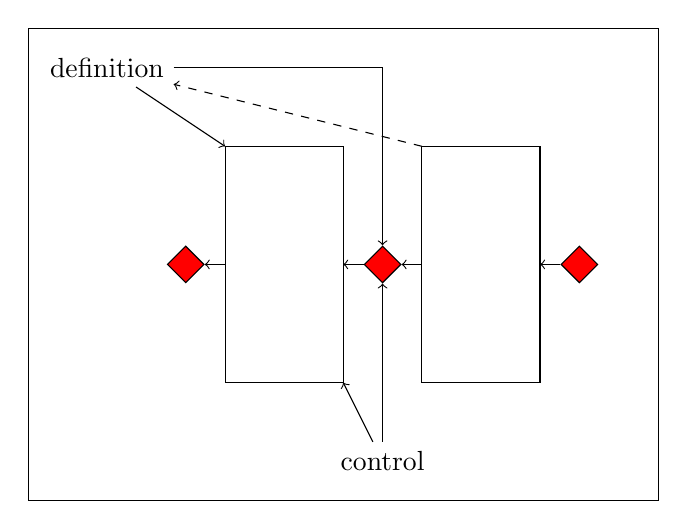
\begin{tikzpicture}
       \draw (-1,-1.5) rectangle (7,4.5);
       \node[draw, diamond,fill=red] (m1) at (1,1.5) {};
       \draw (1.5,0) rectangle (3,3);
       \node[draw, diamond,fill=red] (m2) at (3.5,1.5) {};
       \draw (4,0) rectangle (5.5,3);
       \node[draw, diamond,fill=red] (m3) at (6,1.5) {};
       \draw[->] (m3) -- (5.5,1.5);
       \draw[->] (4,1.5) -- (m2);
       \draw[->] (m2) -- (3,1.5);
       \draw[->] (1.5,1.5) -- (m1);
       \node (def) at (0,4) {definition};
       \node (cont) at (3.5,-1) {control};
       \draw[->] (def) -| (m2);
       \draw[->] (cont) -- (m2);
       \draw[->, dashed] (4,3) -- (def);
       \draw[->] (def) -- (1.5,3);
       \draw[->] (cont) -- (3,0);
    \end{tikzpicture}
    
\end{document}